\begin{name}
{Chuyên ngoại ngữ Hà Nội}
{ĐỀ THI THỬ TỐT NGHIỆP THPT--NĂM 2022 }
\end{name}
\Opensolutionfile{ans}[ngoaingu]
\begin{ex} %Câu 1
Cho cấp số nhân $( {{u}_{n}} )$ với ${{u}_{1}}=5$ và công bội $q=-2$. Giá trị của ${{u}_{2}}$ bằng 
\choice 
{ $7$}
{ \True $-10$}
{ $3$}
{ $-\dfrac{5}{2}$} \end{ex} 
\begin{ex} %Câu 2
Trong không gian $Oxyz$, đường thẳng $\Delta:\heva{
& x=2+2t \\ 
& y=-1+3t \\ 
& z=-4+3t \\ 
}$ đi qua điểm nào dưới đây? 
\choice 
{  $P( 4;2;1 )$}
{ $Q( -2;-7;10 )$} 
{ $N( 0;-4;7 )$}
{ \True $M( 0;-4;-7 )$} \end{ex} 
\begin{ex} %Câu 3
Cho hình chóp $S.ABCD$ có đáy $ABCD$ là hình vuông cạnh $a$. Đường thẳng $SA$ vuông góc với mặt phẳng đáy, $SA=a$. Gọi $E$ là trung điểm của $CD$. Khoảng cách từ $E$ đến mặt phẳng $( SAB )$ bằng
\choice 
{ $\dfrac{a\sqrt{2}}{2}$}
{ \True $a$}
{ $a\sqrt{2}$}
{ $2a$} \end{ex} 
\begin{ex} %Câu 4
Họ nguyên hàm của hàm số $f( x )={{5}^{x}}$ là
\choice 
{ \True $\int {f(x) \mathrm{d} x}=\dfrac{{{5}^{x}}}{\ln 5}+C$}
{ $\int {f( x ) \mathrm{d} x}={{5}^{x}}\ln 5+C$} 
{ $\int {f( x ) \mathrm{d} x}={{5}^{x+1}}+C$}
{ $\int {f( x ) \mathrm{d} x}=\dfrac{5^{x+1}}{x+1}+C$} 
\end{ex} 
\begin{ex} %Câu 5
Với mọi $a;b$ thỏa mãn $3\log a+2\log b=1$, khẳng định nào dưới đây đúng? 
\choice 
{ ${{a}^3}+b^2=1$}
{ \True ${{a}^3}b^2=10$}
{ $3a+2b=10$}
{ ${{a}^3}+b^2=10$} \end{ex} 
\begin{ex} %Câu 6
\immini[thm]{Hàm số nào có đồ thị là đường cong trong hình vẽ bên dưới?
\choice 
{ \True $y=x^4-4x^2+1$}
{ $y=\dfrac{x+1}{x-2}$}
{ $y=x^3+4x^2+1$}
{ $y=2x^2+1$} 
}{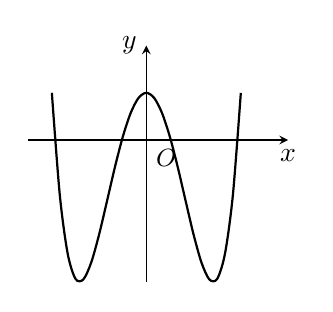
\begin{tikzpicture}[scale=.6]
\draw[-stealth] (-2.5,0) -- (3,0) node[below]{$x$};
\draw[-stealth] (0,-3) -- (0,2) node[left]{$y$};
\draw (0,0) node[below right]{\small $O$};
\draw[thick,smooth] plot[domain=-2:2](\x,{(\x)^4-4*(\x)^2+1});
\end{tikzpicture}}
\end{ex} 
\begin{ex} %Câu 7
Tập xác định của hàm số $y={{( x+2 )}^{\sqrt{2}}}$ là
\choice 
{ $\mathbb{R}\backslash \left\{ -2 \right\}$}
{ \True $( -2;+\infty )$}
{ $( 0;+\infty )$}
{ $\mathbb{R}$} \end{ex} 
\begin{ex} %Câu 8
Diện tích $S$ của mặt cầu bán kính $R$ được tính theo công thức nào dưới đây?
\choice 
{ $\dfrac{3}{4}\pi {{R}^2}$ }
{ $\pi {{R}^2}$ }
{ \True $4\pi {{R}^2}$ }
{ $\dfrac{4}{3}\pi {{R}^3}$ } \end{ex} 
\begin{ex} %Câu 9
Trên mặt phẳng tọa độ, cho $M( 4;-3 )$ là điểm biểu diễn của số phức $z$. Phần ảo của $z$ bằng
\choice 
{ $4$ }
{ $-3i$}
{ $-4$}
{ \True $-3$} \end{ex} 
\begin{ex} %Câu 10
Trong không gian $Oxyz$, cho tam giác $ABC$ có $A(-1;3;2)$, $B(2;0;5)$ và $C(0;-2;1)$. Đường trung tuyến $AM$ của tam giác $ABC$ có phương trình là
\choice 
{ \True $\dfrac{x+1}{2}=\dfrac{y-3}{-4}=\dfrac{z-2}{1}$}
{ $\dfrac{x-1}{2}=\dfrac{y+3}{-4}=\dfrac{z+2}{1}$} 
{ $\dfrac{x+1}{-2}=\dfrac{y-3}{-2}=\dfrac{z-2}{-4}$}
{ $\dfrac{x-1}{-2}=\dfrac{y+3}{-2}=\dfrac{z+2}{-4}$} \end{ex} 
\begin{ex} %Câu 11
Nếu $\int\limits_0^4{f(x)}\,\mathrm{d} x=37$ thì $\int\limits_0^4{[ 2f(x)-3x^2 ]}\,\mathrm{d} x$ bằng
\choice 
{ 12}
{ 18}
{ $-27$}
{ \True 10} \end{ex} 
\begin{ex} %Câu 12
Cho số phức $z$ thoả mãn: $(3+2i)\bar{z}+{{(2-i)}^2}=4+i$. Tổng phần thực và phần ảo của số phức $z$ bằng
\choice 
{ 3}
{ \True 0}
{ 2}
{ 1} \end{ex} 
\begin{ex} %Câu 13
Tiệm cận ngang của đồ thị hàm số $y=\dfrac{2x+1}{x-1}$ là đường thẳng có phương trình
\choice 
{ $x=2$}
{ $y=-2$}
{ $x=1$}
{ \True $y=2$} \end{ex} 
\begin{ex} %Câu 14
Tập nghiệm của bất phương trình ${{3}^{x}}\ge 12$ là
\choice 
{ $[ 4;\,+\infty )$}
{ $( -\infty;\,4 ]$}
{ \True $[ {{\log }_{3}}12;\,+\infty )$}
{ $( -\infty;\,{{\log }_{3}}12 ]$} \end{ex} 
\begin{ex} %Câu 15
Mô đun của số phức $z=4-3i$ bằng'
\choice 
{ \True $| z |=5$}
{ $| z |=7$}
{ $| z |=\sqrt{7}$}
{ $| z |=25$} \end{ex} 
\begin{ex} %Câu 16
Cho hình chóp $S.ABCD$ có tất cả các cạnh đều bằng $a$. Gọi $I$ và $J$ lần lượt là trung điểm của $SC$ và $BC$. Góc giữa hai đường thẳng $IJ$ và $SC$ bằng
\choice 
{ \True $60{}^\circ $}
{ $45{}^\circ $}
{ $90{}^\circ $}
{ $30{}^\circ $} \end{ex} 
\begin{ex} %Câu 17
Cho số phức $z=-3+4i$, khi đó $3z$ bằng 
\choice 
{ \True $z=-9+12i$}
{ $z=-3+12i$}
{ $z=9-12i$}
{ $z=-9+4i$} \end{ex} 
\begin{ex} %Câu 18
Nếu $\int\limits_{2}^5{f( x )\mathrm{d} x}=3$ và $\int\limits_{5}^{7}{f( x )\mathrm{d} x}=9$ thì $\int\limits_{2}^{7}{f( x )\mathrm{d} x}$ bằng
\choice 
{ $6$}
{ $3$}
{ $-6$}
{ \True $12$} \end{ex} 
\begin{ex} %Câu 19
Hàm số nào sau đây đồng biến trên $\mathbb{R}$?
\choice 
{ $y=x+\dfrac{1}{x+3}$}
{ $y=\dfrac{1}{x-2}$} 
{ \True $y=x^3-3x^2+3x+5$}
{ $y=x^4+x^2+1$} \end{ex} 
\begin{ex} %Câu 20
Trong không gian $Oxyz$, cho hai vectơ $\vec{u}=( -1;3;2 )$ và $\vec{v}=( -3;-1;2 )$. Khi đó $\vec{u}.\vec{v}$ bằng
\choice 
{ $3$ }
{ $2$}
{ $10$}
{ \True $4$} \end{ex} 
\begin{ex} %Câu 21
Cho khối lăng trụ đứng có cạnh bên bằng $5$, đáy là hình vuông có cạnh bằng $4$. Thể tích khối lăng trụ đã cho bằng
\choice 
{ $64$ }
{ $20$}
{ $100$}
{ \True $80$} \end{ex} 
\begin{ex} %Câu 22
Trên đoạn $[ -4;\,-1 ]$, hàm số $y=x+\dfrac{9}{x-1}$ đạt giá trị lớn nhất bằng
\choice 
{ \True $-5$}
{ $-\dfrac{29}{5}$}
{ $-\dfrac{11}{2}$}
{ $4$} \end{ex} 
\begin{ex} %Câu 23
Một tổ có 7 nam và 3 nữ. Chọn ngẫu nhiên đồng thời 2 người. Xác suất để 2 người được chọn có ít nhất một nữ bằng
\choice 
{ \True $\dfrac{8}{15}$}
{ $\dfrac{7}{15}$}
{ $\dfrac{1}{15}$}
{ $\dfrac{2}{15}$} \end{ex} 
\begin{ex} %Câu 24
Với mọi số thực $a$ dương khác 1, ${{\log }_{a}}\sqrt[3]{a}$ bằng
\choice 
{ \True $\dfrac{1}{3}$}
{ $3$}
{ $-3$}
{ $0$} \end{ex} 
\begin{ex} %Câu 25
Nếu $\int\limits_{3}^4{f( x )\mathrm{d} x}=3$ thì $\int\limits_{3}^4{-4f( x )\mathrm{d} x}$ bằng
\choice 
{ \True $-12$}
{ $-4$}
{ $12$}
{ $3$} \end{ex} 
\begin{ex} %Câu 26
Trong không gian $Oxyz$, cho điểm $M( -2;1;-1 )$ và đường thẳng $d:\dfrac{x-1}{-3}=\dfrac{y}{2}=\dfrac{z+1}{1}$. Mặt phẳng đi qua $M$ và vuông góc với $d$ có phương trình là
\choice 
{ \True $3x-2y-z+7=0$}
{ $-2x+y-z+7=0$} 
{ $3x-2y-z-7=0$}
{ $-2x+y-z-7=0$} \end{ex} 
\begin{ex} %Câu 27
Cho hàm số $f( x )=x+\cos x$. Khẳng định nào dưới đây là đúng?
\choice 
{ $\int{f( x )\mathrm{d} x}=x\sin x+\cos x+C$}
{ $\int{f( x )\mathrm{d} x}=1-\sin x+C$}
{ \True $\int{f( x )\mathrm{d} x}=\dfrac{x^2}{2}+\sin x+C$}
{ $\int{f( x )\mathrm{d} x}=\dfrac{x^2}{2}-\sin x+C$} 
\end{ex} 
\begin{ex} %Câu 28
Cho khối nón có đường cao $h$ và bán kính đáy $r$. Thể tích của khối nón đã cho được tính bởi công thức nào dưới đây?
\choice 
{ \True $V=\dfrac{1}{3}\pi {{r}^2}h$}
{ $V=\pi {{r}^2}h$}
{ $V=\pi r\sqrt{{{h}^2}+{{r}^2}}$}
{ $V=2\pi r\sqrt{{{h}^2}+{{r}^2}}$} \end{ex} 
\begin{ex} %Câu 29
\immini[thm]{Cho hàm số $y=f( x )$ xác định và liên tục trên đoạn $[ -2\,;\,2 ]$ và có đồ thị là đường cong trong hình vẽ sau. Điểm cực tiểu của đồ thị hàm số $y=f( x )$ là
\choice 
{ $x=1$}
{ $x=-2$}
{ \True $M( 1\,;\,-2 )$}
{ $M( -2\,;\,-4 )$} 
}{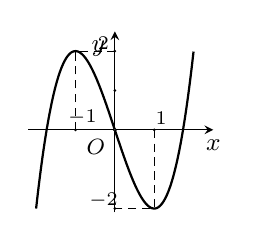
\begin{tikzpicture}[scale=.5]
\draw[-stealth] (-2.2,0) -- (2.5,0) node[below]{\small $x$};
\draw[-stealth] (0,-2.1) -- (0,2.5) node[below left]{\small $y$};
\draw [thin,densely dashed] (-1,0)|-(0,2)  (1,0)|-(0,-2) ;
\draw[thick,smooth,samples=100] plot[domain=-2:2](\x,{(\x)^3-3*(\x)});
\draw [fill=white,draw=black] (0,0) circle (1pt)node[below left]{\footnotesize $O$};
\foreach \x in{-1,1}\draw(\x,0) circle (.5pt) node[shift={(60:5pt)}]{\scriptsize $\x$};
\foreach \y in{-2,2,}\draw(0,\y) circle (.5pt) node[shift={(145:5pt)}]{\scriptsize $\y$};
\end{tikzpicture}}
\end{ex} 
\begin{ex} %Câu 30
Trong không gian $Oxyz$, mặt cầu $( S ):{{( x+1 )}^2}+{{( y-3 )}^2}+{{( z-2 )}^2}=16$ có tâm và bán kính là 
\choice 
{ $I( 1\,;\,-3\,;\,-2 )$ và $R=4$}
{ \True $I( -1\,;\,3\,;\,2 )$ và $R=4$} 
{ $I( 1\,;\,-3\,;\,-2 )$ và $R=16$}
{ $I( -1\,;\,3\,;\,2 )$ và $R=16$} \end{ex} 
\begin{ex} %Câu 31
Nghiệm của phương trình ${{\log }_{3}}( x-2 )=4$ là
\choice 
{ $x=79$}
{ $x=81$}
{ $x=66$}
{ \True $x=83$} \end{ex} 
\begin{ex} %Câu 32
Với $k;n$ là các số nguyên thỏa mãn $0\le k\le n$, công thức nào dưới đây đúng?
\choice 
{ $A_{n}^{k}=\dfrac{n!}{k!( n+k )!}$}
{ \True $A_{n}^{k}=\dfrac{n!}{( n-k )!}$} 
{ $A_{n}^{k}=\dfrac{n!}{k!( n-k )!}$}
{ $A_{n}^{k}=\dfrac{n!}{( n+k )!}$} \end{ex} 
\begin{ex} %Câu 33
Cho khối chóp có diện tích đáy $B$ và chiều cao $h$. Thể tích $V$ của khối chóp đã cho được tính theo công thức vào dưới đây?
\choice 
{ $V=\dfrac{1}{2}Bh$}
{ \True $V=\dfrac{1}{3}Bh$}
{ $V=\dfrac{4}{3}Bh$}
{ $V=Bh$} \end{ex} 
\begin{ex} %Câu 34
Trong không gian $Oxyz$, mặt phẳng $( P ):2x+y-1=0$ có một vectơ pháp tuyến là
\choice 
{ ${{\vec{n}}_{3}}=( 1;2;0 )$}
{ ${{\vec{n}}_{2}}=( 2;1;-1 )$}
{ ${{\vec{n}}_{1}}=( -2;-1;1 )$}
{ \True ${{\vec{n}}_{4}}=( 2;1;0 )$} \end{ex} 
\begin{ex} %Câu 35
Điểm nào sau đây thuộc đồ thị của hàm số $y=x^4-3x^2-5$?
\choice 
{ \True $N( 2;-1 )$}
{  $P( 1;3 )$}
{  $Q( -2;-9 )$}
{  $M( -1;-3 )$} \end{ex} 
\begin{ex} %Câu 36
Đạo hàm của hàm số $y={e^{3x}}$ là
\choice 
{ ${y}'={e^{3x}}$}
{ ${y}'={e^{3x}}.\ln 3$}
{ \True ${y}'=3{e^{3x}}$}
{ ${y}'=\dfrac{{e^{3x}}}{3}$} \end{ex} 
\begin{ex} %Câu 37
Cho hàm số $y=f( x )$ liên tục trên $\mathbb{R}$ và có bảng xét dấu của đạo hàm như sau:
 \\ \centerline{

\begin{tikzpicture}
\tkzTabInit[nocadre,lgt=1.2,espcl=2.2]
{$x$ /.6,$f'(x)$ /.6}
{$-\infty$,$-1$,$0$,$2$,$4$,$+\infty$}
\tkzTabLine{,+,$0$,-,d,+,$0$,-,$0$,+,}
\end{tikzpicture}
}\\
Số điểm cực trị của hàm số đã cho là
\choice 
{ $1$}
{ \True $4$}
{ $3$}
{ $2$} \end{ex} 
\begin{ex} %Câu 38
Cho hàm số $y=f( x )$ có bảng biến thiên như sau:
 \\ \centerline{

\begin{tikzpicture}
\tkzTabInit[nocadre,lgt=1.2,espcl=2.2]
{$x$ /.6,$f'(x)$ /.6,$f(x)$ /1.5}
{$-\infty$,$-2$,$0$,$+\infty$}
\tkzTabLine{,+,$0$,-,$0$,+,}
\tkzTabVar{-/ $-\infty$ ,+/$1$,-/$-3$,+/$+\infty$}
\end{tikzpicture}
}\\
Hàm số đã cho nghịch biến trên khoảng nào dưới đây?
\choice 
{ $( 0;\,+\infty )$}
{ $( -\infty;\,-2 )$}
{ $( -3;\,1 )$}
{ \True $( -2;\,0 )$} \end{ex} 
\begin{ex} %Câu 39
Cho ${{z}_{1}},\,\,{{z}_{2}}$ là hai nghiệm phức của phương trình $3{{z}^2}-7z+27=0$. Giá trị của ${{z}_{1}}|{{z}_{2}} |+{{z}_{2}}| {{z}_{1}}|$bằng 
\choice 
{ $3$}
{ \True $7$}
{ $6$}
{ $9$} \end{ex} 
\begin{ex} %Câu 40
Cho hàm số $y=f( x )$ có đạo hàm $f'( x )=12x^2-2,\,\,\forall x\in \mathbb{R}$. Biết $F( x )$ là một nguyên hàm của $f( x )$ thỏa mãn $F( 0 )=1$ và $F( 1 )=-1$, khi đó $f( 2 )$ bằng 
\choice 
{ $30$}
{ $36$}
{ $-3$}
{ \True $26$} \end{ex} 

\begin{ex} %Câu 42
Trong không gian $Oxyz,$ cho điểm $A( 2;-3;4 )$ và mặt phẳng $( P ):-x+2y+z=0$. Đường thẳng đi qua $A,$ cắt trục $Ox$ và song song với $( P )$ có phương trình là:
\choice 
{ $\dfrac{x-2}{1}=\dfrac{y+3}{2}=\dfrac{z-4}{-3}$}
{ \True $\dfrac{x-2}{2}=\dfrac{y+3}{3}=\dfrac{z-4}{-4}$} 
{ $\dfrac{x}{-2}=\dfrac{y+3}{-3}=\dfrac{z}{4}$}
{ $\dfrac{x+2}{1}=\dfrac{y+11}{2}=\dfrac{z-16}{-3}$} \end{ex} 
\begin{ex} %Câu 43
Cho khối chóp đều $S.ABCD$ có đáy $ABCD$ là hình vuông cạnh $a$. Biết diện tích tam giác $SAC$ là $\sqrt{2}a^2$, thể tích của khối chóp đã cho bằng
\choice 
{ \True $\frac{2}{3} a^{3}$ }
{ $a^{3}$ }
{ $2 \sqrt{2} a^{3}$ }
{ $\frac{4}{3} a^{3}$ } \end{ex} 
\begin{ex} %Câu 44
Cho khối nón đỉnh $S$ có bán kính đáy bằng $\sqrt{3}a $ . Gọi$M$ và $N$ là hai điểm thuộc đường tròn đáy sao cho $MN=2a$. Biết thể tích của khối nón là $\sqrt{2}\pi a^3$ , khoảng cách từ tâm của đường tròn đáy đến mặt phẳng $SMN$  là
\choice 
{ $\dfrac{a}{\sqrt{2}}$ }
{ $2a$ }
{ \True $a$ }
{ $\sqrt{3}a$ } \end{ex} 
\begin{ex} %Câu 45
Có bao nhiêu số nguyên $x$  thỏa mãn $\frac{\sqrt{3-{{\log }_{4}}\left( 2x \right)}}{-{{9}^{x}}+{{10.3}^{x+2}}-729}\le 0$?
\choice 
{ $31$ }
{ \True $29$ }
{ $27$ }
{$28$  }
 \end{ex} 
\begin{ex} %Câu 46
Cho hàm số $f(x)=3x^4+ax^3+bx^2+cx+d$  có ba điểm cực trị là $-2,1,2$. Gọi $y=g(x)$  là hàm số bậc hai có đồ thị đi qua ba điểm cực trị của đồ thị hàm số $y=f(x)$ . Diện tích hình phẳng giới hạn bởi hai đường $y=f(x)$  và $y=g(x)$  có giá trị thuộc khoảng
\choice 
{ $(34;35 )$ }
{ $(36;37 )$ }
{ \True $(37;38 )$ }
{ $(35;36 )$ } \end{ex} 
\Closesolutionfile{ans}